\documentclass[11pt]{article}
\usepackage{fullpage}
\usepackage{graphics,epsfig,color}
\usepackage{wrapfig}
\usepackage{amsmath}
\usepackage{forest}
\usepackage{times}
\usepackage{setspace}
\usepackage{amsmath,amsthm,amssymb}
\usepackage{subfigure}
\usepackage{url}
\newtheorem{problem}{Problem}
\newtheorem{answer}{Answer}
\usepackage{listings}
\usepackage{color}
\usepackage{adjustbox}
\usepackage{tikz}

\definecolor{dkgreen}{rgb}{0,0.6,0}
\definecolor{gray}{rgb}{0.5,0.5,0.5}
\definecolor{mauve}{rgb}{0.58,0,0.82}

\lstset{frame=tb,
	language=Java,
	aboveskip=3mm,
	belowskip=3mm,
	showstringspaces=false,
	columns=flexible,
	basicstyle={\small\ttfamily},
	numbers=none,
	numberstyle=\tiny\color{gray},
	keywordstyle=\color{blue},
	commentstyle=\color{dkgreen},
	stringstyle=\color{mauve},
	breaklines=true,
	breakatwhitespace=true,
	tabsize=3
}

\usetikzlibrary{arrows,trees,positioning}

\tikzset{
	treenode/.style = {align=center, inner sep=-.5pt, text centered,
		font=\sffamily},
	arn/.style = {treenode, circle, white, font=\sffamily\bfseries, draw=black,
		fill=black, text width=2.5em}
}

\begin{document}
\begin{center}
	{\LARGE CSCD320 Homework6}
	
	\bigskip
	
	{\Large Ethan Tuning}
\end{center}

\bigskip

\begin{problem}
\label{prob:1}
 You are given a set of $n$ unit-length tasks, i.e. each task has length $1$. Each task $i$, for $1 \leq i \leq n$, can start at the earliest possible time $r_i$ and must finish by its deadline $d_i$. You are asked to schedule a maximum number of tasks within the given constraint, so that all the picked tasks can be scheduled without conflicts. Describe your strategy on picking what tasks and how to schedule them. Explain why your strategy works.
\end{problem}

\begin{answer}
\label{ans:1}
 For this problem we will need to use the "greedy algorithm" approach to accomplish the task. So we would iterate through all $n$ tasks, at each iteration, if the current task can be fit into the current time interval without missing the deadline, we will then add the current task to the result. If not then we just ignore the current task. This works because as the greedy algorithm is defined it grabs the most optimal solution at that moment, and since we only need to know the best solution at a given point in time then any other way to solve might be slower, or it might be overkill.
\end{answer}

\bigskip

\begin{problem}
\label{prob:2}
 Suppose you are given a text of 97 characters drawn from the alphabet {a, b, c, d, e, f} and the frequency of each letter is:
\begin{center}
\begin{tabular}{ |c|c|c|c|c|c| } 
	\hline
	a & b & c & d & e & f \\
	\hline
	\multirow
	 2 & 10 & 35 & 16 & 25 & 9 \\
	\hline
\end{tabular}	
\end{center}

1. Create a Huffman tree for this text.

2. Show the Huffman code of each letter.

3. Compute the size of the Huffman code compressed version of this text in bits.

4. Calculate te compression ratio: $compressed text size / raw text size$.

\end{problem}

\begin{answer}
\label{ans:2}
The following answers are in order of questions asked in the above problem.

1. 
\begin{center}
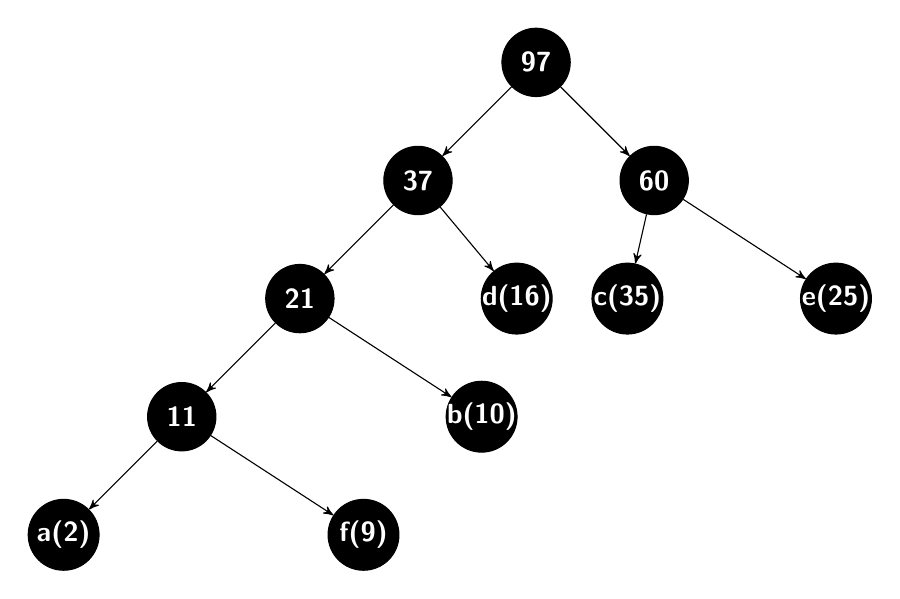
\begin{tikzpicture}[->,>=stealth',level/.style={sibling distance = 3cm,
	level distance = 1.5cm}] 
\node [arn] {97}
child{ node [arn] {37}
	child{ node [arn] {21}
		child{ node [arn] {11}
			child{ node [arn] {a(2)}}
			child{ node [arn, right = 1em] {f(9)}}
		}
		child{ node [arn, right = 1em] {b(10)}}
	}
	child{ node [arn, right = -2em] {d(16)}}
}
child{ node [arn,] {60}
	child{node [arn, right = 2em] {c(35)}}
	child{node[arn, right = 1em] {e(25)} node[above right= 2em and -1em] {} node[right = 1em]{} }	
}; 
\end{tikzpicture}
\end{center}

2.

a: 0000

b: 001

c: 10

d: 01

e: 11

f: 0001

\bigskip

3.

17 bits

\bigskip

4.

$17/776 = 0.021907$
\end{answer}

\bigskip

\begin{problem}
\label{prob:3}
Consider a directed graph arranged into rows and columns. Each vertex is labeled
$(j, k)$, where row $j$ lies between $0$ and $M$, and column $k$ lies between $0$ and $N$. The start vertex is $(0, 0)$ and the destination vertex is $(M,N)$. Each vertex $(j, k)$ has an associated weight $W(j, k)$. The weight of a path is defined as the summation of the weights of all the vertices on that path. There are edges from each vertex $(j, k)$ to at most three other vertices: $(j + 1, k)$, $(j, k + 1)$, and $(j + 1, k + 1)$, provided that these other vertices exist.

That is, the input of your algorithm is a simple 2d array W of size $(M + 1) × (N + 1)$ using 0-based indexing, where each array element is a number, which can be positive, negative, or zero. The goal of your algorithm is to count the number of different paths from $(0, 0)$ to $(M, N)$ that have MINIMUM total weight.

1. Provide a recursive formula that computes the exact value that is specified in the problem. (Refer to the book chapter for examples of recursive formulas, which essentially is to precisely describe the recursive structure in the solution.)

2. Express the recursive formula as a bottom-up table-driven dynamic programming
algorithm, and determine its running time.
\end{problem}

\begin{answer}
\label{ans:3}
The following answers are in order of questions asked in the above problem.

1. Recursive formula: $minWeight(m, n) = min (minWeight(m-1, n-1), minWeight(m-1, n), minWeight(m, n-1)) + weight[m][n]$

2. $total[i][j] = min(total[i-1][j-1], total[i-1][j], total[i][j-1]) + total[i][j]$ will be called after we have created the first row and first column. Time cost will be $O(mn)$
\end{answer}

\bigskip

\begin{problem}
\label{prob:4}
Search and learn three existing algorithms that use the dynamic programming strategy, in addition to those that we have discussed the class (“rod-cutting” and “matrix-chain”). For each algorithm, in your own language, concisely and clearly describe:

1. The problem statement.

2. The main idea of the solution. Where is the recursive structure in the solution?

3. Why recursion-based idea does not work?

4. Why dynamic programming works?

5. The source of your finding.
\end{problem}

\begin{answer}
\label{ans:4}
 1. Edit Distance algorithm - given two strings, str1 and str2, as well as 3 operations (insert, replace, and remove) can be done only on the str1. Find the smallest number of operations that str1 can have done on it to be turned into str2. The solution is if the str1 is empty, insert all characters from the str2. If str2 is empty remove all characters from str2. If last characters are same, ignore and continue through string. If the last characters are different then we have to find all possibilities. With recursion this would take FOREVER, because we would be doing a lot of the same work over and over. Dynamic works because it saves info as we go within the same array space. I found this list and chose all my examples from this list. https://www.quora.com/What-are-the-top-10-most-popular-dynamic-programming-problems-among-interviewers
 
 \bigskip
 
 2. Maximum size square sub-matrix with all 1's - given a binary matrix, find out the max size square sub-matrix that contains only 1's. For this we will iterate over each row considering each is a histogram, and finding the maximum of those. Then if current element is a 1 add it to the result array. Then just return the size of the resulting array. Recursion cannot work because there would not be anyway to access the previous results. Dynamic works because we are working with the same array the whole time and just building the result form it.
 
 \bigskip
 
 3. Longest increasing subsequence size - given an array of numbers. Find the longest subsequence in that array. If the current element is the smallest among the elements in the current list, start a new list of length 1. Then, if the current is the largest, then copy the largest active list, and extend it by the current element. If the current element is in between then find the largest that is smaller then the current element. Copy and extend the list, then discard the other lists of the same size. Recursion will again, be slow. Dynamic makes the solution must faster because again we are not solving the same things we know over and over.
 
 \bigskip
 
 A lot of dynamic algorithms are there because recursion costs time and space. Almost all of these algorithms will have similar feel so its kind of hard to elaborate on them in depth. Dynamic programming does the same thing as other solutions, it just is usually a better way for time and space issues in computing. Not just with algorithms, is dynamic a great  way to do things but with other aspects of programming too. Creating things at runtime, allocating at runtime, and much more are examples at which dynamic ideas are the best way to do things. 
\end{answer}
\end{document}